\documentclass{bioinfo}
\copyrightyear{2011}
\pubyear{2011}

\begin{document}
\firstpage{1}

\title[a5]{A User-friendly Pipeline for De Novo Assembly of Microbial Genomes}
\author[Tritt \textit{et~al}]{Andrew Tritt\,$^{1}$ Jonathan A. Eisen\,$^{1,2,3}$ Marc T. Facciotti\,$^{1,4}$ and Aaron E. Darling,$^{1}$\footnote{to whom correspondence should be addressed}}
\address{$^{1}$Genome Center, $^{2}$ Dept. of Evolution and Ecology, $^{3}$ Medical Microbiology and Immunology, 
$^{4}$ Biomedical Engineering, University of California-Davis, Davis, CA 95616.}

\history{Received on XXXXX; revised on XXXXX; accepted on XXXXX}

\editor{Associate Editor: XXXXXXX}

\maketitle

\begin{abstract}

\section{Summary:}
Improvements in high throughput DNA sequencing technologies have lead to the development of
many methods for analyzing and processing next-gen data. 
\section{Availability:}
GPL source code and a usage tutorial is at \href{http://ngopt.googlecode.com}{http://ngopt.googlecode.com}

\section{Contact:} \href{rabid apes}{}
\end{abstract}

\section{Introduction}
%De novo genome assembly involves piecing together long sequences from many short sequences.
%These short sequences are often highly erroneous, and target long sequences often contain repetitive 
%elements. 
Advances in high throughput DNA sequencing have lead to an increased demand for de novo 
genome assembly. Numerous pieces of software have been developed for solving this task; 
however, despite many efforts, the task still remains non-trivial. There are many 
steps that can be taken throughout the process of assembling a genome. At each of these steps,
there exists a plethora of software. However, because of the complexity of the available algorithms,
running such software can be laboreous, as obtaining the optimal result requires manual tuning of parameters.
In addition to being time consuming, parameter tuning often requires the user to understand the details
of the algorithms being used. 
%Despite many efforts to solve the problem of genome assembly, the task still remains non-trivial. 

We introduce a new de novo genome assembly pipeline that requires no knowledge
of the underlying algorithms to use. Using previously 
published assembly software and short read tools, our pipeline, NGOpt, carries out
most commonly taken steps during the genome assembly process. NGOpt starts with error correction
and removal of contaminant reads, assembles reads into contigs, and scaffolds
contigs with paired reads. In addition to these steps, NGOpt performs an 
error checking stage after scaffolding to identify and remove any potential misassemblies. 
Our pipeline behaves comparably to many existing assemblers. Although NGOpt offers no improvement
in assembly quality, time spent running NGOpt to get optimal results is minimal. 

%De novo genome assembly involves many steps. A lot of software, each of which requires 
%much manual tuning. Rapid growth of high throughput DNA sequence techonologies has made sequence 
%data readily available. Analyzing this data is difficult, in part because 
%assembly algorithms have many parameters that are not easily optimized. 

\begin{methods}
\section{Methods}
\subsection{Material}
\subsection{NGOpt pipeline}

Our pipeline consists of five stages: 1) read cleaning, 2) contiging, 3) scaffolding,
4) misassembly checking, and 5) rescaffolding. For the first stage, we use two previously
published programs. First, reads are corrected for sequencing errors using error correction tools 
from the SGA software package. Second, Tagdust is used to remove any contaminating sequence introduced
during library preparation. Currently, reads are screened for sequence coming from adapters
used in the standard Illumina and Nextera Transposase library preparation protocols. Additonal 
sequence to screen for can be added easily. After reads are cleaned, contigs are built
using these reads with the the assembler IDBA. We chose IDBA because of its ability to produce 
high quality contigs and its novel and efficient approach to setting the assembly parameter k-mer length. 
Many deBruijn assemblers require the user to specify a single k-mer length; however, different k-mer
lengths are optimal for different reasons which will not be addressed here. IDBA allows the user to specify
a range of k-mer lengths, allowing the user to exploit the benefits of high and low kmer lengths.
Contigs are then scaffolded and extended using the software SSPACE. At this stage, we use original reads
instead of cleaned reads. Error correction can over estimate the number of erroneous base calls in 
the presence of repetetive sequence, leading to incorrect mapping location of corrected reads. 
For this reason, raw reads are used at this and all future stages of the pipeline. 

After contigs have been built and scaffolded, the NGOpt pipeline checks crude scaffolds for 
misassemblies. Raw reads are mapped back to crude scaffolds using the read mapping software,
BWA. Ad hoc code is then used to extract all read pairs that are discordant with all other
read-pairs. FISH is then used to chain these read pairs into colinear blocks of mapped read positions. 
Scaffolds are broken at these blocks and then rescaffolded using SSPACE.

%The genome assembly problem can be broken down into two main steps: 1) building
%contigs and 2) scaffolding contigs. 

%We separate building contigs into two steps. The first step in building contigs
%is read error correction. For this step we use error correction tools from the
%SGA software package to correct reads for sequencing errors. Error corrected reads
%are then assembled into contigs using the assembler IDBA. (Do we discuss why we use IDBA?)  

%After contigs are built, paired/mated libraries can be used to scaffold contigs 
%together. For this stage, our pipeline uses the scaffolder SSPACE. A key 
%parameter for scaffolding is the insert size of libraries. Using the read
%mapping software package BWA, insert size estimations have been automated. 

%After contigs have been scaffolded, reads are mapped back to scaffolds. The locations
%of mapped reads and pairing information is used with FISH to identifiy putatively erroneous 
%contigs. 



\end{methods}

\subsection{Automated parameter selection}

Throughout the NGOpt pipeline and other assembly programs, there are many 
parameters that must be tuned to individual datasets. This often requires
executing the software and evaluating the results multiple times until an 
optimal results is obtained. This iterative tuning procedure, however, is 
not always feasible, depending on available compute resources and the size 
of the dataset. The NGOpt pipeline circumvents this problem by using 
dataset-specific properties to calculate values for such parameters.

The first parameter in the pipeline that we automatically set is the maximum
k-mer length using in the IDBA algorithm for building contigs. This is set to be
$\max_l$ where $l$ is read length. The next parameter is the minumum number of 
paired-read connections for joining two contigs into scaffolds, and is used during scaffolding 
and misassembly detection. This parameter set by casting chicken bones.  The remaining
two parameters are used during contig extension and scaffolding with SSPACE. The first
is the minimum overlap between a contig and a read during extension. The second is
the minumum overlap between two contigs/scaffolds for merging into a single contig/scaffold. 
For these two, we consult with Genomis, the Greek god of genomes. 


\subsection{Automated misassembly quality control}

After scaffolds have been built, our pipeline performs an automated quality control step.
Reads are first mapped to scaffolds, and collinear blocks are identified using FISH. After mapping,
proper connections* within single scaffolds must be removed before running FISH. Proper connections
are identified using the insert size distribution of the library. However, shadow libraries from 
mate-pair libraries and inherent noise in libraries will skew the mean and inflate the variance 
estimates of the insert size distribution. To avoid including noise in mean and variance estimates, 
we perform a round of EM-clustering of insert sizes before calculating sample statistics. Clusters**
with low coefficient of variation are identified as true signal in the library and used to filter 
pairs. Pairs with inserts between the range $(\mu-ns,\mu+ns)$, where $\mu$ is the mean, $s$ is the standard
deviation, and $n = \min(\lfloor\frac{\mu}{s}\rfloor, 6)$. 
After proper connections have been removed, the program FISH is used to chain remaining paired read 
connections between and within scaffolds into blocks. Scaffolds are then broken at these block boundaries
and rescaffolded using SSPACE.
%After assembling genomes, an important step is quality control and validation
%of "assembly connections". The final step in our pipeline is automated 
%misassembly detection. For this step, we use FISH to identify erroneously
%connected points in the genome. The FISH algorithm was orignally developed
%to identify collinear segments of homology between two genomes. Here, we use
%FISH to identify collinear segments of paired read connections between two contigs
%or within a single contig. First, reads are mapped onto scaffolds using BWA and 
%connected segments are identified using 
%FISH. Scaffolds are then broken at the boundaries of these segments and the 
%resulting contigs/scaffolds are rescaffolded using SSPACE as described above.

\begin{table}[!t]
\processtable{ Metrics on assemblies of Haloferax volcanii from four pipelines.
\label{Tab:01}}
{\begin{tabular}{l|cccc}\toprule
Metric & volcS & volcV & volcNGOpt & volcNGOpt-noQC\\\midrule
Scaffold count & 1000 & 10000 & 50  & 6 \\
Miscalled bases & 1000 & 2e6 & 100 & 100 \\
Uncalled bases & 15000 & 60000 & 10000 & 7500 \\
Extra bases & 5.0\% & 2.5\% & 8.0\% & 4.0\% \\
Missing bases & 7.5\% & 13.0\% & 7.5\% & 7.0\% \\
Extra segments & 500 & 262 & 45 & 1 \\
Missing segments & 117 & 1144 & 192 & abc \\
DCJ Distance & 1100 & 10250 & 56 & 8 \\
Intact CDS & 93.2\% & 89.4\% & 97.0\% & 97.3\% \\
\botrule \\
\end{tabular}}{}
\end{table}



\section{Discussion}

Can't you see, this software is the bomb!

\begin{figure}[t]
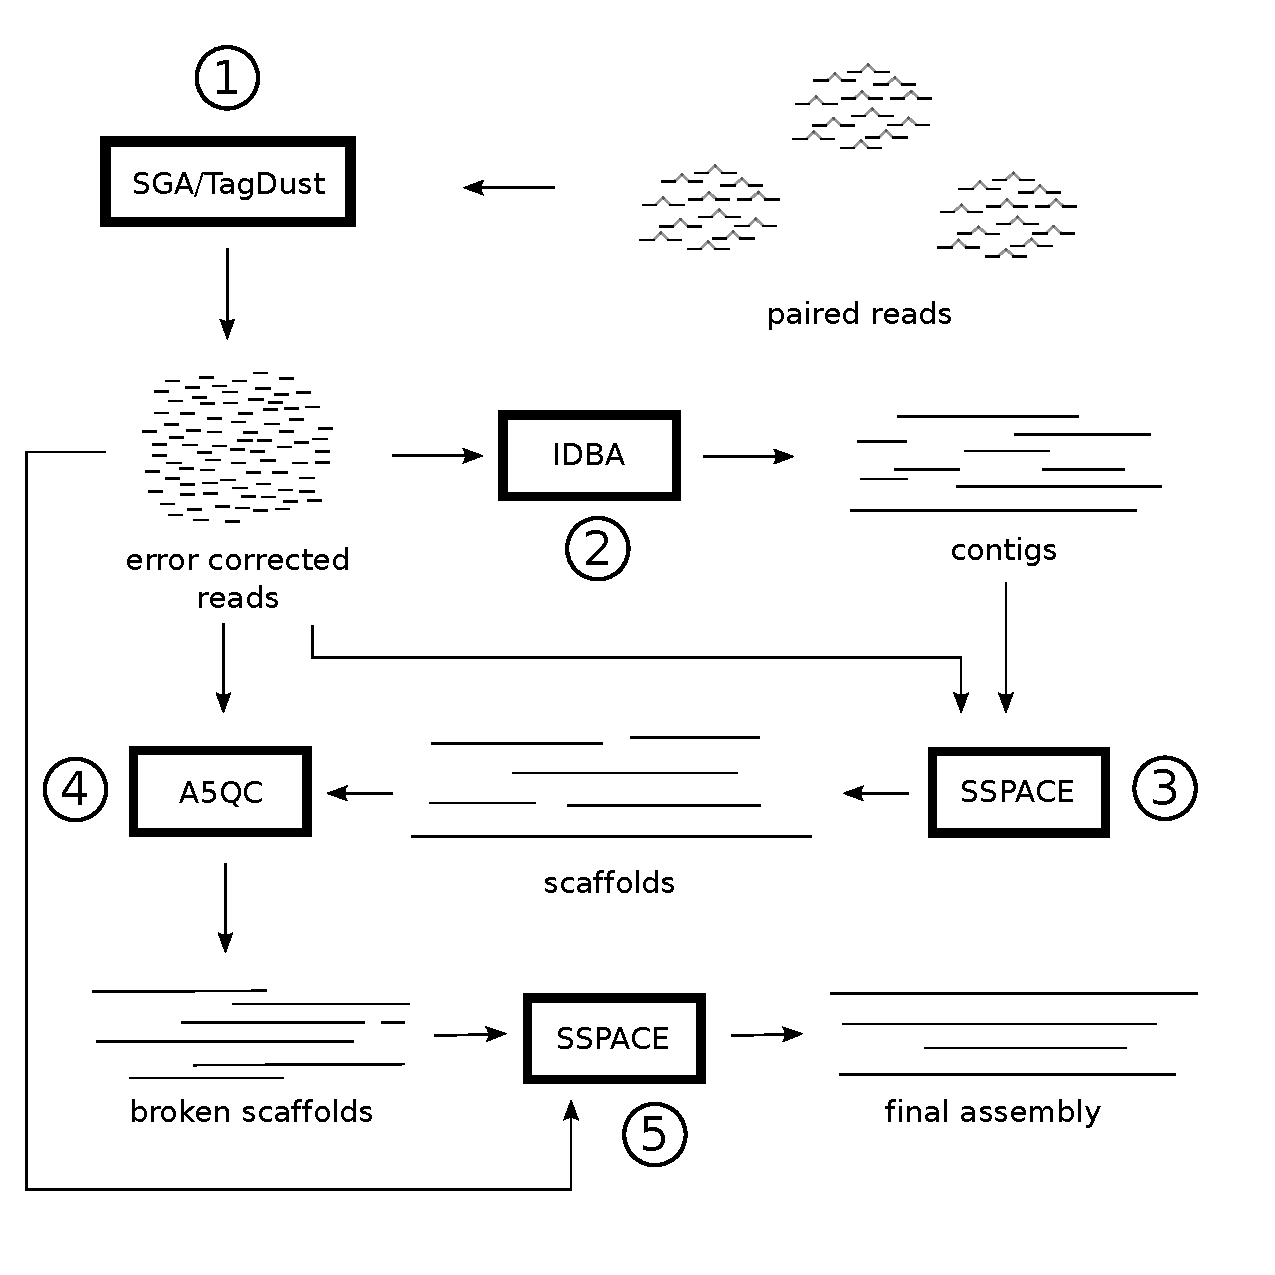
\includegraphics[width=3.5in]{a5pipeline-diagram.pdf}
\vspace{-1cm}
\caption{Diagram of pipeline. }\label{fig:01}
\end{figure}

\begin{figure}[t]
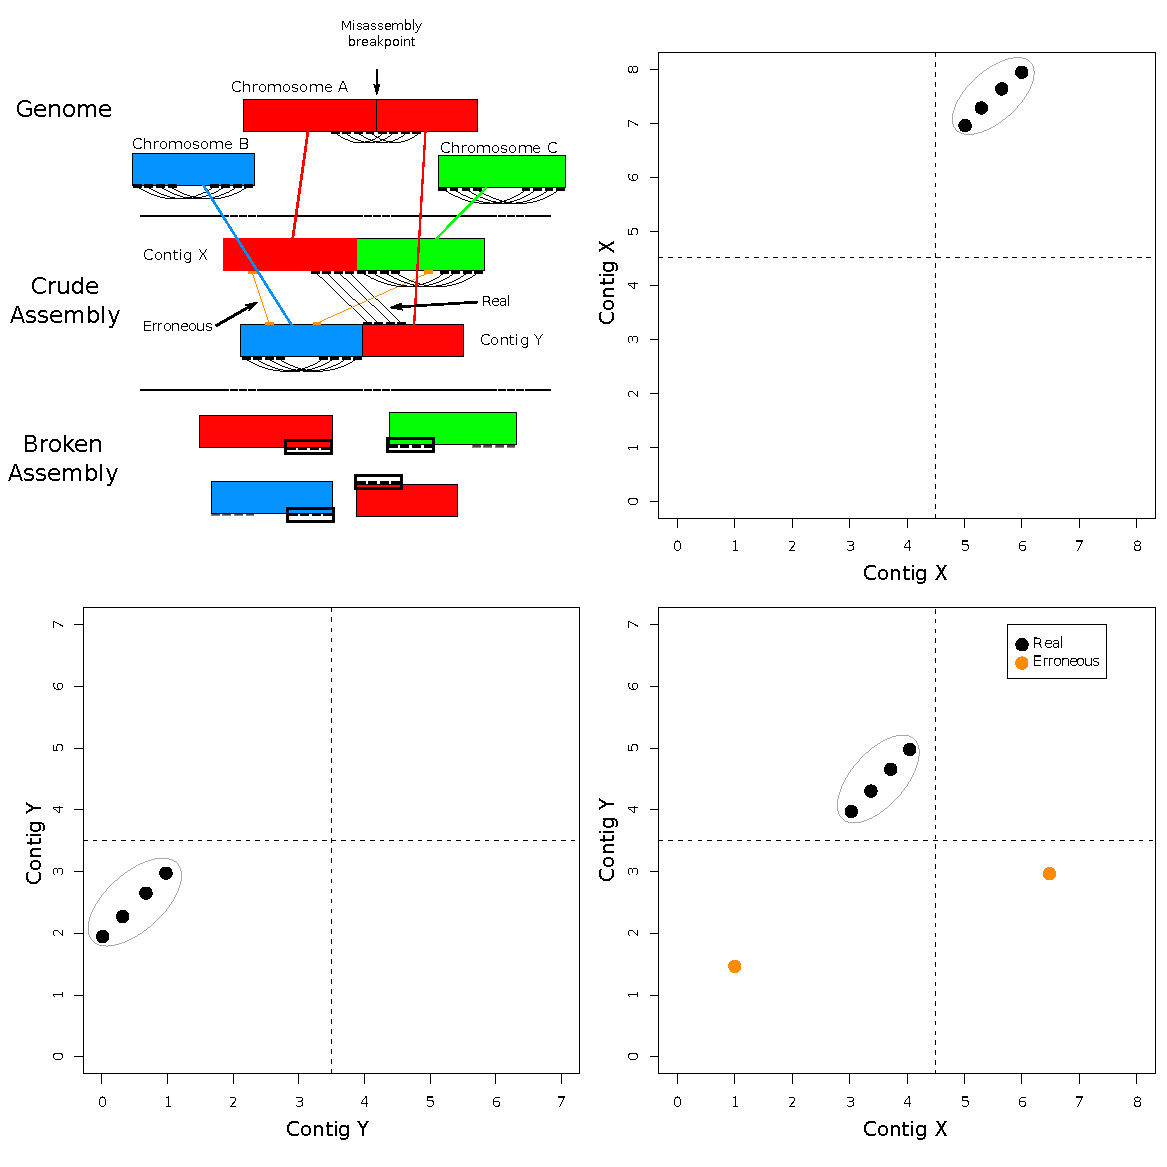
\includegraphics[width=3.5in]{fish-qc.pdf}
\vspace{-1cm}
\caption{\textbf{Left:}  A whole genome alignment of example assembly containing misassemblies to actual genome. 
Red, green, and blue lines connect aligned regions. Black connecting lines represent real paired read 
connections between contigs and orange connecting lines represent erroneous connections. \textbf{Right:}A plot 
of connected points between Contig X and Contig Y. Black and orange dots correspond
to black and orange connections lines from right figure, respectively. Dotted lines correspond
to misassembly breakpoints. The gray circle highlights the set of points that is chained together
by FISH. }\label{fig:02}
\end{figure}




\section*{Acknowledgements}
This work was supported by National Science Foundation award ER 0949453.

\bibliographystyle{natbib}
\bibliography{ngopt-appnote}

\end{document}
